%------------------------------------------------------------------------------
%   PACKAGES AND OTHER DOCUMENT CONFIGURATIONS
%------------------------------------------------------------------------------

\documentclass[twoside,twocolumn]{article}

%\usepackage[sc]{mathpazo} % Use the Palatino font
%\usepackage[T1]{fontenc} % Use 8-bit encoding that has 256 glyphs
%\linespread{1.05} % Line spacing - Palatino needs more space between lines
%\usepackage{microtype} % Slightly tweak font spacing for aesthetics

\usepackage[english]{babel} % Language hyphenation and typographical rules

% Document margins
\usepackage[hmarginratio=1:1,top=32mm,left=20mm,right=20mm,columnsep=20pt]{geometry}
% Custom captions under/above floats in tables or figures
\usepackage[hang, small,labelfont=bf,up,textfont=it,up]{caption}
\usepackage{booktabs} % Horizontal rules in tables

\usepackage{enumitem} % Customized lists
\setlist[itemize]{noitemsep} % Make itemize lists more compact
\usepackage{textcomp}

% Allows abstract customization
\usepackage{abstract}
% Set the "Abstract" text to bold
\renewcommand{\abstractnamefont}{\normalfont\bfseries}
% Set the abstract itself to small italic text
\renewcommand{\abstracttextfont}{\normalfont\small\itshape}

\usepackage{fancyhdr} % Headers and footers
\pagestyle{fancy} % All pages have headers and footers
\fancyhead{} % Blank out the default header
\fancyfoot{} % Blank out the default footer
\fancyhead[C]{\thetitle}
\fancyfoot[RO,LE]{\thepage} % Custom footer text

\usepackage{titling} % Customizing the title section

\usepackage{hyperref} % For hyperlinks in the PDF
\usepackage{amsmath}

\usepackage{tikz}
\usetikzlibrary{bayesnet}
\usetikzlibrary{arrows}

\usepackage{color}
\usepackage{caption}
\usepackage{subcaption}

\usepackage{graphicx}

\captionsetup[figure]{labelfont={bf},textfont=normalfont}

%------------------------------------------------------------------------------
%   TITLE SECTION
%------------------------------------------------------------------------------

\setlength{\droptitle}{-4\baselineskip} % Move the title up

\pretitle{\begin{center}\Huge\bfseries} % Article title formatting
\posttitle{\end{center}} % Article title closing formatting

\title{MT Project Proposal: \\ Using Neural Networks to Learn Word Alignments}
\author{%
\textsc{Bailey Parker} \\[1ex]
\normalsize Johns Hopkins University \\
\normalsize \href{mailto:bailey@jhu.edu}{bailey@jhu.edu}
 \and
 \textsc{Vivian Tsai} \\[1ex]
\normalsize Johns Hopkins University \\
\normalsize \href{mailto:vtsai5@jhu.edu}{vtsai5@jhu.edu}
 \and
  \textsc{William Watson} \\[1ex]
\normalsize Johns Hopkins University \\
\normalsize \href{mailto:wwatso13@jhu.edu}{wwatso13@jhu.edu}
}

\date{}%\today} % Leave empty to omit a date
% \renewcommand{\maketitlehookd}{%

% }

%------------------------------------------------------------------------------
\DeclareMathOperator*{\argmax}{arg\,max}
\newcommand{\qdist}[1]{\ifmmode\langle#1\rangle\else\textlangle#1\textrangle\fi}


\begin{document}

% Print the title
\maketitle

%------------------------------------------------------------------------------
%   ARTICLE CONTENTS
%------------------------------------------------------------------------------

% \section{Introduction}

% TODO

%------------------------------------------------

\begin{abstract}
% \noindent \blindtext
We seek to explore the word alignment problem with the help of neural networks. More specifically, we want to see if the original Expectation-Maximization (EM) approach to word alignment can be transcribed as a neural network in a supervised and unsupervised setting.
\end{abstract}

% REMEMBER IDEA IS TOO COPY PROPOSAL INTO FINAL WRITEUP

\section{Introduction}
% WHAT IS OUR METRIC!!!
Word Alignment seeks to match individual words in a parallel corpus such that the Alignment Error Rate (AER) is minimized. In a previous assignment, our task was to implement IBM Model 1, based on the Expectation-Maximization (EM) algorithm. Following IBM Model 1, we implemented a reparametrization of IBM Model 2 that favors alignments along the diagonal. Finally, we implemented an Alignment by Agreement Model that trained a French to English and English to French model and combined the results to make better alignments.

Our proposal for this project is to replace the EM algorithm and reparametrization of IBM Model 2 with a neural network architecture. In addition, the model will incorporate Alignment by Agreement. We will use PyTorch to build the model and loss functions. The key concept is that we can create a loss function that the network will learn the optimal parameters to learn word alignments from a corpus of parallel text.


\section{Background}
Our approach is inspired by current research in topic modeling with Latent Dirichlet Allocation (LDA) models. LDA models are generative probabilistic models that model topics across distributions of words in a corpus. LDAs are based on variational methods and EM for Bayes parameter estimation.

applying a NN to approximate the posterior distributions.
see apibm - apply tech to lda.
\footnote{\url{http://www.jmlr.org/papers/volume3/blei03a/blei03a.pdf}}

% INSERT GRAPHIC OF PLATE DIAGRAM FOR LDA HERE!
% Also cite LDA paper.
\begin{figure*}
\centering
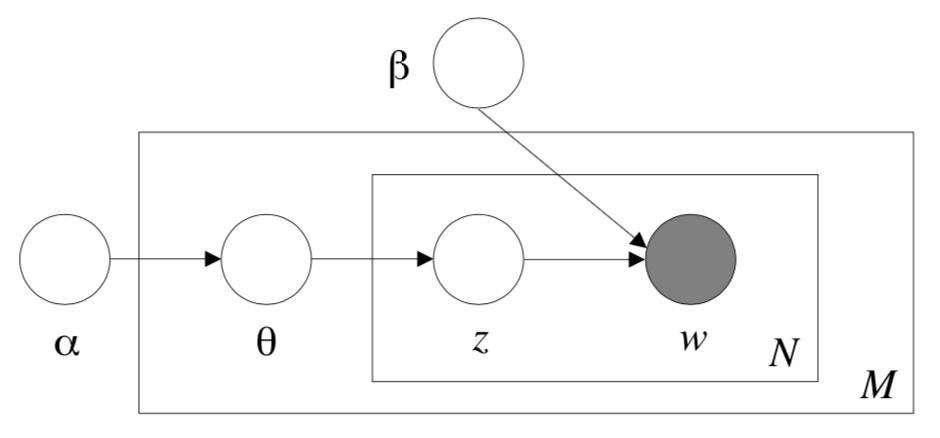
\includegraphics[scale=0.5]{LDADiagram}
\caption{Graphical model representation of LDA. The boxes are “plates” representing replicates. The outer plate represents documents, while the inner plate represents the repeated choice of topics and words within a document. }
\end{figure*}

Current research attempts to supplant the probabilistic modeling with a neural network architecture. 

Additional inspiration comes from Variational Auto-Encoders (VAE).
% Expand discussion on VAE and similiarity to our proposal. MAybe include VAE diagram.

\section{Original Formulation}
% Can steal shorten version from original paper! yay!

\section{Our Formulation}
% basically regurtiate (nicely) what was on board. Maybe make fancy diagrams and stuff.
% also embeddings, positional, POS tagging, etc.

% alignment distirbution, i is target position, j is source position, lambda and null p_0
\begin{equation}
a(i, j, \lambda, p_0) =
\begin{cases} 
      p_0 & \text{if } null \\
     (1-p_0) \cdot e^{-\lambda | \frac{i}{m} - \frac{j}{n}|} & \text{else}
   \end{cases}
\end{equation}


\begin{figure}
\centering
\begin{tikzpicture}

  % Define nodes
  \node[obs]                               (y) {$t$};
  \node[latent, above=0.75cm of y] (a) {$a$};
  \node[latent, above=0.75cm of a, xshift=-0.6cm] (w) {$\lambda$};
  \node[latent, above=0.75cm of a, xshift=0.6cm]  (x) {$p_0$};
  \node[obs, right=0.75cm of y]            (t) {$s$};
  \node[latent, below=0.95cm of y]            (theta) {$\theta$};

  % Connect the nodes
  \edge {x,w} {a} ; %
  \edge {a,t} {y} ; %
  \edge {theta} {y} ; %

  % Plates
  \plate [xscale=1.75, yscale=1.25] {y} {(a)(y)} {$\quad$} ;

\end{tikzpicture}
\caption{Probabilistic Plate Diagram for Word Alignment, where $t$ is target, $s$ is source, $\theta$ is the translation probability, $\lambda$ is a position parameter, $p_0$ is the null probability, and $a$ is the alignment distribution.}
\end{figure}

\section{Data}
% talk about subtitle extraction. Also labeling of data for supervised? Or should that go in supervised trainign section. Get Bailey to metnion Nikita metric for baseline on unaligned corpus.

\section{Training}

\subsection{Supervised Training}
% cut out top half of model, talk about how we will label our data and incoropoate

\subsection{Unsupervised Training}
% 5 term loss function

\section{Expectation}
% Our Hopes and Dreams!


\begin{equation}
\centering
\begin{split}
\textit{le chat} &\mapsto \textit{the cat} \\
\textit{est} &\mapsto \textit{is} \\
\textit{noir} &\mapsto \textit{black} \\
\end{split}
\end{equation}



\begin{figure}
\centering
\begin{tabular}{ |l|l| }
  \hline
  \multicolumn{2}{|c|}{Baseline Decoder Experiments} \\
  \hline
  Experiment & \multicolumn{1}{|c|}{Score} \\
  \hline
  Default & -1439.87 \\
  High Stack ($s=10K$) & -1436.36 \\
  High Probability ($k=200$) & -1374.87\\
  Both & -1353.25 \\
  \hline
\end{tabular}
\caption{Baseline Beam Search Decoding Scores}
\end{figure}

\begin{figure*}[ht]
\centering
\begin{tabular}{ |l|l|l|l| }
  \hline
  \multicolumn{4}{|c|}{Scoring Results Per Model} \\
  \hline
  Model & \multicolumn{1}{|c|}{Score} & \multicolumn{1}{|c|}{$\mu$} & \multicolumn{1}{|c|}{$\sigma$} \\
  \hline
  Baseline ($k=1$, $s=1$) & -1439.87 & -30.00 & 13.71 \\
  Baseline ($k=200$, $s=10K$) & -1353.25 & -28.19 & 13.07 \\
  \hline
  Phrase Insertion ($k=200$, $s=1K$) & -1259.07 & -26.23 & 11.44 \\
  + Position Distortion ($\lambda=0.005$) & -1261.23 & -26.28 & 11.50 \\
  + Post Process Reordering & -1255.53 & -26.16 & 11.43 \\
  + Lemmatization Model & \multicolumn{1}{|c|}{N/A} & \multicolumn{1}{|c|}{N/A} & \multicolumn{1}{|c|}{N/A} \\
   \hline
   Markov Chain Monte Carlo Simulation ($iter=20K$) & -1499.58 & -31.24 & 14.54 \\
  \hline
  Final Model & -1255.48 & -26.16 & 11.46 \\
  \hline
\end{tabular}
\caption{Model Scores with Average and Standard Deviation}
\end{figure*}

\end{document}
